\newpage
\section*{Ziel}
Aufbau sowie Funktion eines Lock-In-Verstärkers untersuchen.

\section{Theorie}
\label{sec:theorie}

Ein Lock-In-Verstärker beinhaltet einen integrierten phasenempfindlichen Detektor.
Er wird zur Messung von stark verrauschten Signalen verwendet.
Dafür wählt man eine Referenzfrequen $\omega_0$, mit derer das Messignal moduliert wird.
\begin{figure}[H]
    \centering
    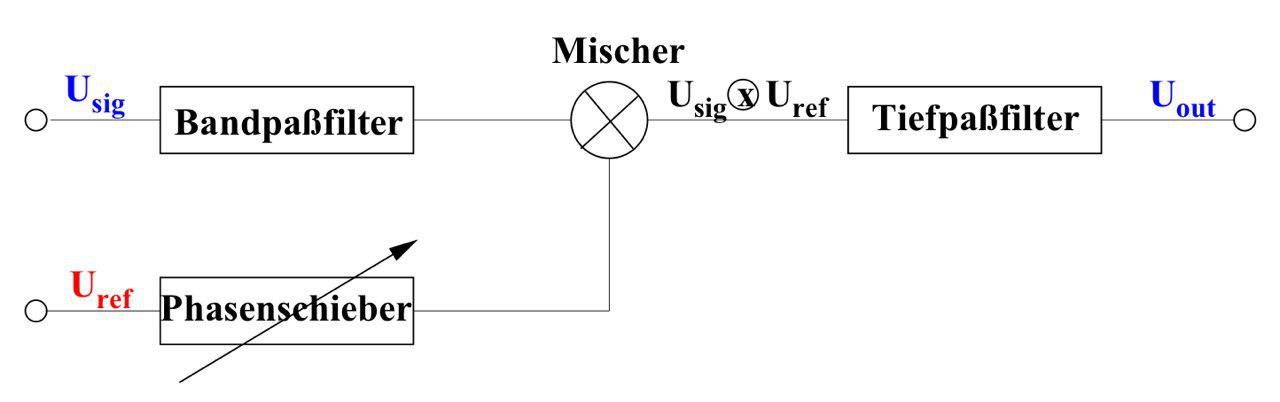
\includegraphics[width=0.8\textwidth]{bilder/aufbau_schema.jpg}
    \caption{Schematischer Aufbau eines Lock-In-Verstärkers \cite[1]{Anleitung}}
    \label{fig:aufbau_generell}
\end{figure}

Hauptbestandteil sind dabei Bandpassfilter (lässt nur Signale eines bestimmten Bandpasses passieren),
Phasenschieber, Mischer und ein Tiefpassfilter (lässt Signale unterhalb der Grenzfrquenz passieren).
\subsection{Funktionsweise}

Basis ist ein verrauschtes Nutzsignal $U_{sig}$. Dieses Signal
passiert zu erst den Bandpassfilter, der die Rauschanteil um $\omega_0$ entfernt.
Dies wird im Mischer mit einem Referenzsignal $U_{ref}$ mit der Frequen $\omega_0$ multipliziert.
Dabei kann über den Phasenschieber die Phasenlage $\Phi$ reguliert werden, sodass
die Signale synchronisiert werden können ($\Delta \Phi=0$).
Im nachfolgenden integriert der Tiefpass das Mischsignal und mittelt Rauschbeträge
heraus. Schließlich gilt für das Ausgangssignal:
\begin{equation}
    U_{out} \propto U_0 \;\textrm{cos}\;\Phi
\end{equation}
Die Bandbreite des Rauschens,kann durch die Zeitkonstante $\tau=RC$
des Tiefpasses beliebig klein variiert werden.
Dieses Kompination verbessert die Güte um das 100fache, gegenüber einem
einfachen Bandpass.